% !TEX program = xelatex
\def\NN{\mathbb{N}}
\def\RR{\mathbb{R}}
\def\ZZ{\mathbb{Z}}
\def\QQ{\mathbb{Q}}
\def\PP{\mathcal{P}}
\def\SS{\mathcal{S}}
\def\DD{\mathcal{D}}
\def\sub{\setminus}
\def\bld{\mathbf}
\def\lmf{\lim_{n \to \infty}}
% Make the ref command use parenthesis
\let\oldref\ref
\renewcommand{\ref}[1]{(\oldref{#1})}

\newcommand{\ontop}[1]{\overset{\text{#1}}}
\newcommand{\ang}[1]{\langle #1 \rangle}
\newcommand{\pip}[1]{\left| #1 \right|}



% style
\newcommand{\bm}[1]{\displaystyle{#1}}
\def\nl{$ $ \newline}

\ExplSyntaxOn

\NewDocumentCommand{\getenv}{om}
{
  \sys_get_shell:nnN{ kpsewhich ~ --var-value ~ #2 }{}#1
}

\ExplSyntaxOff

%environments

\documentclass{article}
\usepackage{amsmath,mathtools,enumerate,xparse,centernot,polyglossia,graphicx}
\usepackage[utf8]{inputenc}
\usepackage[a4paper, margin=1.1in]{geometry}
\usepackage[]{amsthm} %lets us use \begin{proof}
\usepackage[makeroom]{cancel}
\usepackage[]{amssymb} %gives us the chA \mathcal{R} Acter \varnothing
% \usepackage[frak=mma]{mathalfa}
\setdefaultlanguage{hebrew}
\setotherlanguage{english}
\usepackage{fontspec}
%\setmainfont{Frank Ruehl CLM}
\setmainfont{David CLM}
\setmonofont{Miriam Mono CLM}
\setsansfont{Simple CLM}
\DeclarePairedDelimiter\set\{\}
% Use the following if you only want to change the font for Hebrew
%\newfontfamily\hebrewfont[Script=Hebrew]{David CLM}
%\newfontfamily\hebrewfonttt[Script=Hebrew]{Miriam Mono CLM}
%\newfontfamily\hebrewfontsf[Script=Hebrew]{Simple CLM}
\getenv[\ID]{ID}
\graphicspath{ {./} }

\title{אינפי 2 - ממ"ן 11}
\author{אליחי טורקל \ID}
\date\today

%\clearpage %Gives us a page break before the next section. Optional.
%\selectlanguage{english}
	%Section and subsection automatically number unless you put the asterisk next to them.

\begin{document}
	\maketitle %This command prints the title based on information entered above

	\section*{שאלה 1}
	נגדיר $f(x) = x - \flr{x}$
	\subsection*{סעיף א}
	הראו כי $f$ אינטגרבילית בכל קטע $[a,b]$ אך אין לה קדומה באף קטע שאורכו גדול מ-1.
	\begin{proof}
		ידוע ש $\flr{x}$ רציפה בכל $x \not \in \ZZ$ ולכן בכל מקטע $[a,b]$ היא רציפה למקוטעין בכל הקטע חוץ מב $x \in \ZZ$, \\
		וע"כ רציפה בכל הקטע למעט מספר סופי של נקודות וממשפט 1.19 היא אינטגרבילית ב $[a,b]$, \\
		 וכמובן ש $f(x) = x$ רציפה בכל $\RR$ ומכלל הלינאריות של אינטגרביליות נובע ש $f(x) = x + \flr{x}$ אינטגרבילית בקטע $[a,b]$. \\
		 ומכיוון שכל הנקודות אי רציפות של $\flr{x}$ הן ממין ראשון אזי $f(x)$ לא יכולה להיות נגזרת של אף פונקציה, מכיוון שנקודות האי רציפות של נגזרת הן ממין שני בלבד, ועל כן אין ל $f(x)$ פונקציה קדומה.
	\end{proof}

	\subsection*{סעיף ב}
	לכל $x > 0$ מצאו את הביטוי המפורש עבור $F(x) = \int_0^x f(t) \,dt$
	\begin{proof}
		גרף הפונקציה הוא בעצם אוסף קווים ישרים עם שיפוע 1 מ $y = 0$ ועד $y = 1$ וחוזר חלילה (מכיוון שזה רק החלק השברי)
		ולכן בעצם השטח שמתחת לכל מקטע הוא משולש ישר זווית עם בסיס באורך 1 וגובה בגודל 1 וע"כ שטח המשולש הוא $\frac{1}{2}$ \\
		מתכונת האדיטיביות של האינטגרל המסויים אנו מקבלים:
		\[
			F(x) = \int_0^x f(t) \,dt = \int_0^{\flr{x}} f(t) \,dt + \int_{\flr{x}}^x f(t) \, dt
		\]
		האינטגרל הראשון הוא בעצם $\frac{1}{2}$ כפול מספר המשולשים בגרף, ז"א $\frac{\flr{x}}{2}$. \\
		האינטגרל השני הוא השטח של המשולש ה"קטן" האחרון, ואותו נחשב בעזרת גובה כפול בסיס שהם בעצם שווים מכיוון שהשיפוע של היתר הוא 1 וע"כ השטח של אותו המשולש הוא: $\frac{\left(x - \flr{x}\right)^2}{2}$ ובס"הכ:
		\[
			F(x) = \frac{\flr{x}}{2} + \frac{\left(x - \flr{x}\right)^2}{2}
			= \boxed{\frac{\flr{x} + \left(x - \flr{x}\right)^2}{2}}
		\]
	\end{proof}

	\pagebreak
	\subsection*{סעיף ג}
	הוכיחו כי $1 \leq \int_2^6 f(x) \sin \frac{\pi}{x} \, dx \leq 2$
	\begin{proof}
		יהי $x \in [2,6]$, מתקיים:
		\[
		2 \leq x \leq 6
		\Rightarrow
		\frac{1}{6} \leq \frac{1}{x} \leq \frac{1}{6}
		\Rightarrow
		\frac{\pi}{6} \leq \frac{\pi}{x} \leq \frac{\pi}{6}
		\Rightarrow
		\sin \frac{\pi}{6} \leq \sin \frac{\pi}{x} \leq \sin \frac{\pi}{6}
		\Rightarrow
		\boxed{\frac{1}{2} \leq \sin \frac{\pi}{x} \leq 1}
		\]
		ולכן מתוך המונוטוניות של האינגרל המסויים נקבל ש:
		\setcounter{equation}{0} \begin{align}
			\int_2^6 f(x) \frac{1}{2} \, dx \leq
			\int_2^6 f(x) \sin \frac{\pi}{x} \, dx \leq
			\int_2^6 f(x) 1 \, dx \\
			\int_2^6 f(x) \frac{1}{2} \, dx = (F(6) - F(2)) \cdot \frac{1}{2} = \frac{3 - 1}{2} = 1 \\
			\int_2^6 f(x) 1 \, dx = F(6) - F(2) = \frac{3 - 1}{2} = 1 \\
			1 \leq \int_2^6 f(x) \sin \frac{\pi}{x} \, dx \leq 2
		\end{align}
	\end{proof}


	\section*{שאלה 2}
	תהי $f(x)$ פונקציה אינטגרבילית וחיובית בקטע $[a,b]$. \\
	הוכיחו שאם הפונקציה $\frac{1}{f(x)}$ חסומה ב-$[a,b]$, אז היא אינטגרבילית בקטע זה.
	\begin{proof}
		נסמן $g(x) = \frac{1}{f(x)}$
		לפי הנתון קיים חסם עליון $\mathfrak{M} > g(x)$ ומכיוון ש $f(x)$ חיובית אזי גם $\frac{1}{f(x)}$ חיובית וגם $\mathfrak{M} > 0$. \\
		ולכל חלוקה של $[a,b]$ מתקיים $M_i(g) = sup \, g([x_{i-1}, x_i]) = \frac{1}{inf \, f([x_{i-1}, x_i])}$ וגם \\
		$m_i(g) = inf \, g([x_{i-1}, x_i]) = \frac{1}{sup \, f([x_{i-1}, x_i])}$. \\
		ומכאן נסתכל על התנאי לאינטגרביליות של $g(x)$ לפי דארבו:
		\[
		\sum_{i=1}^n \brac{M_i(g) - m_i(g)} \Delta x_i =
		\sum_{i=1}^n \brac{\frac{1}{M_i(f)} - \frac{1}{m_i(f)}} \Delta x_i =
		\sum_{i=1}^n \frac{M_i(f) - m_i(f)}{M_i(f)m_i(f)} \Delta x_i
		\]
		ומכיוון ש $\mathfrak{M} > \frac{1}{f(x)}$ אזי:
		\[
			\sum_{i=1}^n \frac{M_i(f) - m_i(f)}{M_i(f)m_i(f)} \Delta x_i  <
			\mathfrak{M} \cdot \mathfrak{M} \sum_{i=1}^n \brac{M_i(f) - m_i(f)} \Delta x_i
		\]
		וקיבלנו בעצם ש $\sum_{i=1}^n \brac{M_i(g) - m_i(g)} \Delta x_i < \mathfrak{M}^2 \sum_{i=1}^n \brac{M_i(f) - m_i(f)} \Delta x_i$. \\
		ולכן לפי 1.10 אם $f(x)$ אינטגרבילית אזי קיים $\varepsilon > 0$ כך ש:
		\[\sum_{i=1}^n \brac{M_i(g) - m_i(g)} \Delta x_i < \mathfrak{M}^2 \sum_{i=1}^n \brac{M_i(f) - m_i(f)} \Delta x_i < \varepsilon\]
		ולכן אם $f(x)$ אינטגרבילית אזי $g(x) = \frac{1}{f(x)}$ גם אינטגרבילית.

	\end{proof}

	\pagebreak
	\section*{שאלה 3}
	תהי $f(x)$ פונקציה רציפה ב-$[0, \infty)$ המקיימת $\int_0^{x^2(1+x)} f(t) \, dt$ לכל $x > 0$ חשבו את $f(2)$.

	\begin{proof}
		f(x) רציפה ב $[0, \infty)$ ובפרט ב $[0, a]$ לכל $a > 0$, ולכן ממשפט 1.33 נובע כי $F'(x) = f(x)$. \\
		נסמן $F(c) = \int_0^c f(t) \, dt$ ונקבל ש $F(x^2(1+x)) = x$ ולכן:
		\[
			F(x^2(1+x))' = x' \Rightarrow
			(2x + 3x^2) \cdot f(x^2(1+x)) = 1
		\]
		נפתור את $x^2(1 + x) = 2$ ונקבל ש $x=1$, נציב במשוואה ונקבל $(2+3) \cdot f(2) = 1 \Rightarrow \boxed{f(2) = \frac{1}{5}}$.
	\end{proof}

	\section*{שאלה 4}
	הוכיחו הפריכו.
	\subsection*{סעיף א}
	אם $f$ בעלת נגזרת רציפה בקטע $[0, 1]$ ו- $\int_0^1 f(x) \, dx = 1$, אז $\int_0^1 x f'(x) \, dx = f(1) - 1$.
	\begin{proof}
		נשתמש באינטגרציה בחלקים, ונציב $u = x$, $u' = 1$ ו $v = f$, $v' = f'$ ונקבל
		\[ \int_0^1 u(x)v'(x) \, dx = \int_0^1 x f'(x) \, dx \overset{(a)}=  1 \cdot f(1) - 0 \cdot f(0) - \int^1_0 f(x) \, dx \overset{(b)}= f(1) - 1 \]
		(a) - הנוסחא היסודית ביחד עם אינטגרציה בחלקים \\
		(b) - נתון ש $\int^1_0 f(x) \, dx = 1$
	\end{proof}

	\subsection*{סעיף ב}
	אם $f(x)$ רציפה ב-$\RR$ת אז לכל $a \in \RR$ מתקיים $\limf{t}{0}\frac{1}{t}\int_{a-t}^{a+t} f(x) \, dx = 2f(a)$.
	\begin{proof}
		נפצל את האינטגרל לפי משפט 1.23:
		\[
			\int_{a-t}^{a+t} f(x) \, dx
			 = \int_{a-t}^{a} f(x) \, dx + \int_{a}^{a+t} f(x) \, dx
		\]
		נניח ש $f(x)$ רציפה, ולכן ממשפט 1.29 נקבל שקיים $c_1 \in [a-t, a]$ ו $c_2 \in [a, a+t]$ ככה ש:
		\setcounter{equation}{0} \begin{align}
			\frac{1}{a - a + t}\int^a_{a-t} f(x) = f(c_1) \Rightarrow
			\int^a_{a-t} f(x) = t \cdot f(c_1) \\
			\frac{1}{a + t - a}\int^{a+t}_{a} f(x) = f(c_2) \Rightarrow
			\int^{a+t}_{a} f(x) = t \cdot f(c_2)
		\end{align}
		נחבר חזרה ונקבל:
		\begin{align*}
			\int_{a-t}^{a+t} f(x) \, dx
			= \int_{a-t}^{a} f(x) \, dx + \int_{a}^{a+t} f(x) \, dx
			= t \cdot f(c_1) + t \cdot f(c_2) =
			t(f(c_1) + f(c_2))
		\end{align*}
		נכפיל ב $\frac{1}{t}$:
		$\frac{1}{t} \int_{a-t}^{a+t} f(x) \, dx = f(c_1) + f(c_2)$ \\
		ומכיוון ש $c_1 \in [a-t, a]$, $c_2 \in [a, a+t]$ אזי כאשר $t \to 0$ נקבל ש $c_1 = c_2 = a$ ולכן:
		\[
			\limf{t}{0} \frac{1}{t} \int_{a-t}^{a+t} f(x) \, dx
			= \limf{t}{0} f(c_1) + f(c_2)
			= f(a) + f(a)
			= \boxed{2f(a)}
		\]
	\end{proof}

	\subsection*{סעיף ג}
	קיימת פונקציה $f(x)$ אינטגרבילית בקטע $[0, 2]$ ומקיימת את התנאים הבאים לכל $t \in [1,2]$:
	\[
		\int^t_0 f(x) \, dx \neq t, \,
		\int^2_0 f(x) \, dx > 2, \,
		\int^1_0 f(x) \, dx < 1
	\]
	\begin{proof}
		נסמן $F(u) = \int^u_0 f(x) \, dx$ ונגדיר $g(u) = F(u) - u$ שהיא רציפה כסכום רציפות,
		בעזרת הנתונים נקבל ש:
		\begin{align*}
			g(1) = F(1) - 1 = \int^1_0 f(x) - 1 \leq 0 \\
			g(2) = F(2) - 2 = \int^2_0 f(x) - 2 \geq 0
		\end{align*}
		ממשפט 5.29 באינפי 1 נקבל שקיים $c \in (1,2)$ כך ש $g(c) = 0$
		בעצם: $g(c) = F(c) - c = 0$ ולכן $F(c) = c$ כנדרש.
	\end{proof}

	\section*{שאלה 5}
	נסמן ב-$S$ את השטח הכלוא בין העקומה $y = e^{-x}$ לישר $y=x$ בקטע $[0,1]$. \\
	הראו כי ${S = \frac{3}{2} + \frac{1}{e} - 2\alpha - \alpha^2}$ כאשר $\alpha$ פתרון המשוואה $x + \ln x = 0$.
	\begin{proof}
		\[
			x + \ln x = 0 \Rightarrow
			\ln x = -x \Rightarrow
			\ln x = \ln e^{-x} \Rightarrow
			x = e^{-x}
		\]
		שתי הפונקציות הנתונות: $y = x$, $y = e^{-x}$ נפגשים בנקודה $x = e^{-x}$ שזה בעצם כאשר $x = \alpha$(מכיוון שהראינו ש $x + \ln x = 0 $ שקול ל $x = e^{-x}$).
		מכיוון שהפונקציות חותכות זו את זו בקטע נחשב בנפרד את השטח כשהראשונה מעל השניה והשטח כשהשניה מעל הראשונה, וביחד:
		\setcounter{equation}{0} \begin{align}
			\int e^{-x} - x \,dx = -e^{-x} - \frac{x^2}{2} \\
			\int x - e^{-x} \,dx = \frac{x^2}{2} + e^{-x} \\
			\int_0^{\alpha} e^{-x} - x \,dx + \int_{\alpha}^1 x - e^{-x} \,dx =
			-e^{-\alpha} - \frac{\alpha^2}{2} + e^0 - \frac{0^2}{2} + \frac{1^2}{2} + e^{-1} - \frac{\alpha^2}{2} - e^{-\alpha} = \\
			-2e^{-\alpha} - \alpha^2 + \frac{3}{2} + e^{-1} =
			\boxed{\frac{3}{2} + \frac{1}{e} - 2\alpha - \alpha^2}  \nonumber
		\end{align}
	\end{proof}

	\pagebreak
	\section*{שאלה 6}
	באיור מתואר סגמנט פרבולי בעל בסיס $2a$ וגובה $h$, כלומר, התחום המוגבל על ידי ציר ה-$y$
	והפרבולה שעליכם למצוא את משוואתה (שתלויה כמובן בפרמטרים חיוביים $a$ ו $h$). \\
	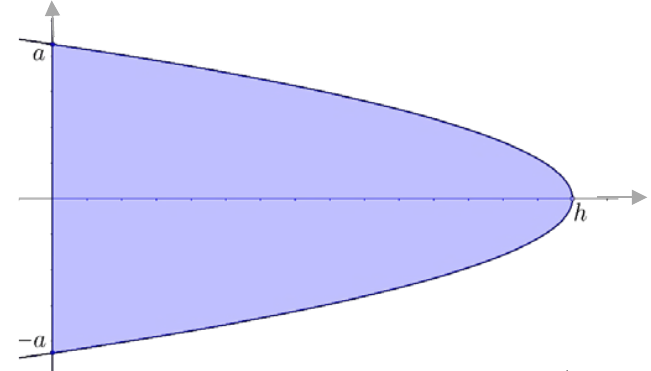
\includegraphics[scale=0.45]{parabolic-segment}

	\subsection*{סעיף א}
	מצאו את השטח של התחום
	\begin{proof}
		נסתכל על פרבולה שחותכת את ציר ה $x$ בנקודות $x = a$, $x = -a$ ואת ציר ה $y$ בנקודה $y = h$. \\
		ומכיוון שפרבולה זה בעצם פולינום ממעלה שניה, אזי מהמשפט היסודי של האלגברה אנו יודעים שיש לכל היותר 2 שורשים לפולינם שהם בעצם $x = \pm a$
		ולכן הפולינום נראה ככה: $f(x) = C(x - a)(x + a)$ כאשר $C$ הוא קבוע שלא תלוי ב $x$ (אחרת קיים עוד שורש ואז לא נקבל פרבולה). \\
		מתוך הנתון של $y = 0$ אנו למדים ש $f(0) = h$ אזי אם נציב נקבל ש:
		\[
		f(0) = C(0 - a)(0 + a)
		= -Ca^2 = h \Rightarrow
		C = - \frac{h}{a^2}
		\]
		נציב חזרה ונקבל: $f(x) = -\frac{h}{a^2}(x - a)(x + a)$ נפשט ונקבל: $f(x) = h\brac{1 - \brac{\frac{x}{a}}^2}$ נחשב את השטח בעזרת אינטגרל מסויים:
		\[
		\int f(x) \, dx = h\brac{x - \frac{x^3}{3a^2}}
		\]
		נשתמש בנוסחא היסודית ונקבל:
		\begin{align*}
		\int_{-a}^a f(x) =
		h\brac{a - \frac{a^3}{3a^2}} - h\brac{-a - \frac{(-a)^3}{3a^2}}
		&= h \brac{2a - \frac{2a^3}{3a^2}} \\
		&= h \brac{2a - \frac{2a}{3}}
		= h \brac{\frac{6a - 2a}{3}}
		= \boxed{\frac{4a}{3}h}
	\end{align*}
	\end{proof}

	\subsection*{סעיף ב}
	מצאו את נפח הגוף הנוצר מסיבוב של התחום הזה סביב ציר ה-$x$.
	\begin{proof}
		נחליף את $x$ ו $y$ ע"מ לקבל את משוואת הסגמנט המקורית (ולא הפרבולה שיצרנו ע"י הפיכת הצירים)
		\begin{align*}
			x = h\brac{1 - \brac{\frac{y}{a}}^2} \Rightarrow
			\frac{x}{h} = 1 - \brac{\frac{y}{a}}^2 \Rightarrow
			\brac{\frac{y}{a}}^2 = 1 - \frac{x}{h} \Rightarrow
			y^2 &= a^2(1 - \frac{x}{h}) \\
			y &= \sqrt{a^2(1 - \frac{x}{h})} \Rightarrow
			\boxed{y = a\sqrt{1 - \frac{x}{h}}}
		\end{align*}
		נשתמש בנוסחה מעמוד 60 לחישוב נפח של גוף סיבוב:
		\begin{align*}
			&\int \pi \brac{a\sqrt{1 - \frac{x}{h}}}^2
			= \int \pi a^2 \brac{1 - \frac{x}{h}}
			= \pi a^2 \brac{x - \frac{x^2}{2h}} \\
			&V = \int^h_0 \pi f(x)^2
			= \pi a^2 \brac{h - \frac{h^2}{2h}}
			= \boxed{\pi a^2 \frac{h}{2}}
		\end{align*}
	\end{proof}

\end{document}
